\documentclass[12pt]{book}
\usepackage[utf8]{inputenc}
\usepackage[spanish]{babel}
\usepackage{listings}
\usepackage{graphicx}

\begin{document}

\section{Singleton}

\subsection{Problema}

Descripción del problema típico que normalmente se resuelva con el patrón. 

Por ejemplo en el caso de Singleton:
Existe una clase que sólo puede tener una instancia, esta clase típicamente guarda información global para todo el sistema que no debe repetirse o tener múltiples valores. Por esta razón se busca que la clase tenga únicamente una instancia.

Lorem ipsum dolor sit amet, consectetur adipiscing elit, sed eiusmod tempor incidunt ut labore et dolore magna aliqua. Ut enim ad minim veniam, quis nostrud exercitation ullamco laboris nisi ut aliquid ex ea commodi consequat. Quis aute iure reprehenderit in voluptate velit esse cillum dolore eu fugiat nulla pariatur. Excepteur sint obcaecat cupiditat non proident, sunt in culpa qui officia deserunt mollit anim id est laborum.


\subsubsection{Ejemplos}
Archivo de configuración (bolsas de propiedades)
Canales de comunicación (JNDI, etc...)
Administrador de conexión con una DBMS
Etc...

\subsection{Intención}

Descripción breve de cómo el patrón pretende resolver el problema. Abstraída de detalles de implementación, la intención describe el enfoque o el algoritmo que el patrón utiliza para tratar el comportamiento problemático.

Por ejemplo en el caso de Singleton:
El patrón previene la creación de instancias adicionales, típicamente una primera instancia es creada al momento en que el sistema se inicializa, aunque esto no es obligatorio. El patrón utiliza accesos estáticos para que los otros módulos se comuniquen con la única instancia... etc...

Agregar en esta sección imágenes ilustrativas, o ejemplos.

\begin{figure}[h]
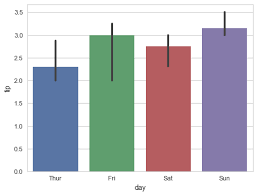
\includegraphics[width=8cm]{imagenes/index.png}
\end{figure}

Lorem ipsum dolor sit amet, consectetur adipiscing elit, sed eiusmod tempor incidunt ut labore et dolore magna aliqua. Ut enim ad minim veniam, quis nostrud exercitation ullamco laboris nisi ut aliquid ex ea commodi consequat. Quis aute iure reprehenderit in voluptate velit esse cillum dolore eu fugiat nulla pariatur. Excepteur sint obcaecat cupiditat non proident, sunt in culpa qui officia deserunt mollit anim id est laborum.

\newpage
\subsection{Solución}

Descripción breve de los detalles de implementación del patrón, ya en un lenguaje más técnico, incluir un diagrama de clases:

\begin{figure}[h]
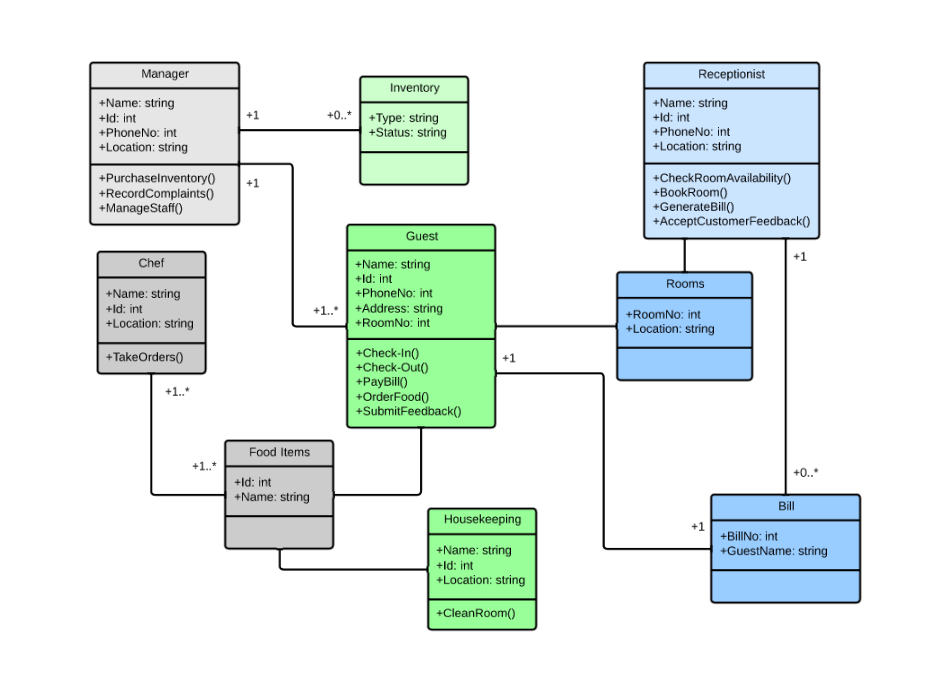
\includegraphics[width=8cm]{imagenes/uml.PNG}
\end{figure}

Se implementa una clase que contiene una referencia estática a sí misma. Esta referencia típicamente es privada, y se accede por medio de métodos estáticos que encapsulan los llamados a la implementación.

% Singleton tiene la peculiaridad que tiene varias implementaciones alternativas, la clásica, la ingenua y la segura 
\textbf{Implementación clásica:} \\

Explicación: Lorem ipsum dolor sit amet, consectetur adipiscing elit, sed eiusmod tempor incidunt ut labore et dolore magna aliqua. Ut enim ad minim veniam, quis nostrud exercitation ullamco laboris nisi ut aliquid ex ea commodi consequat. Quis aute iure reprehenderit in voluptate velit esse cillum dolore eu fugiat nulla pariatur.

\begin{verbatim}
public class Registro {
	
    private static Registro puntero = null;
    
    private ArrayList<Integer> id_jugadores;
    
    private Registro() {
        id_jugadores = new ArrayList<Integer>();
    }
    
    public void agregarJugador(int id) {
        id_jugadores.add(id);
    }
    
    public ArrayList<Integer> getId_jugadores() {
        return id_jugadores;
    }
    
    public void mostarJugadores() {
        System.out.println(id_jugadores.toString());
    }
    
    public static Registro solicitarReferencia() {

        if (puntero == null) {
            puntero = new Registro();
        }   
        return puntero;
    }
}
\end{verbatim}

\textbf{Implementación ingenua:} \\
Explicación: Lorem ipsum dolor sit amet, consectetur adipiscing elit, sed eiusmod tempor incidunt ut labore et dolore magna aliqua. Ut enim ad minim veniam, quis nostrud exercitation ullamco laboris nisi ut aliquid ex ea commodi consequat. Quis aute iure reprehenderit in voluptate velit esse cillum dolore eu fugiat nulla pariatur.

\begin{verbatim}
public class Matemática {
	
    public int mcd (int a, int b) {
        if (b == 0) {
            return a;
        }
        else {
            return mcd(b, a % b);
        }
    }
    
    public int mcm (int a, int b) {
        return (a * b) / mcd(a, b);
    }
}
\end{verbatim}

\newpage

\textbf{Caso de prueba:} \\
Explicación: Lorem ipsum dolor sit amet, consectetur adipiscing elit, sed eiusmod tempor incidunt ut labore et dolore magna aliqua. Ut enim ad minim veniam, quis nostrud exercitation ullamco laboris nisi ut aliquid ex ea commodi consequat. Quis aute iure reprehenderit in voluptate velit esse cillum dolore eu fugiat nulla pariatur.

\begin{verbatim}
public class Marcador {
    public static void main(String[] args) {
    
        Registro jugadores = Registro.solicitarReferencia();
    
        jugadores.agrgarJugador(1);
        jugadores.agrgarJugador(2);
    
        Registro copia_jugadores = Registro.solicitarReferencia();
    
        copia_jugadores.agrgarJugador(3);
        copia_jugadores.agrgarJugador(4);
        
        jugadores.mostarJugadores();
        copia_jugadores.mostarJugadores();	
    }
}
\end{verbatim}


\subsection{Opcional: Antipatrón}
Descripción breve de cómo el patrón puede ocasionar más problemas que soluciones. Por ejemplo la implementación segura de Singleton típicamente funciona como un antipatrón, generando problemas de rendimiento al requerir demasiadas verificaciones o sincronización innecesarias.

Esto no significa que la implementación segura de Singleton sea un antipatrón, como todo en patrones, depende de la naturaleza del problema. Más que nada prevenir una implementación inadecuada del patrón.
\end{document}
